\section{Budget} % income and outlays
The budget for the first year of the open data lab has a scope consisting of a purchase order for AWS time and personnel detailed from the Data Science Institute.

\begin{center}
Table of Income and Outlays for 2018-2019

\begin{tabular}{lccr}
\hline
\hline
Source & Time (FTE) & Time (hours) & USD \\
\hline
\multicolumn{4}{c}{Income} \\
\hline
DSI Funds & && 10,000 \\
HM Funds & && 475 \\
Data Scientist & 1/2 & & \\
Clark Lab Dev & & 80 & \\
DSI Staff & & 100 & \\
\hline
Total Income & 1/2  & 180 & 10,475 \\
\hline
\hline
\multicolumn{4}{c}{Outlays} \\
\hline
AWS & && 897 \\
Personnel Assigned & 1/2  &  & \\
Personnel Temporary & & 180 & \\
\hline
Total Outlays & 1/2  & 180 & 897 \\
\hline
\hline
Net & 0 & 0 & 5578 \\
\hline
\hline
\end{tabular}
\end{center}

\subsection{Income}
\begin{itemize}
\item Cash: The DSI allocated \$10,000 for computation and storage from AWS from the period of April 1, 2018 - May 31, 2019. These funds are drawn from PTAO 147242.102.LC00112.30002.
\item Cash: The Healthy Markets research project used ODL services for computation and storage on AWS. The ODL is authorized to transfer cost in proportion to the Healthy Markets PTAO 147412.107.DR03397.30002.
\item Personnel: The DSI allocated 50\% of a staff Data Scientist's time to the ODL project (1/2 FTE). The Clark lab contributed 80 hours of software developer time.
\end{itemize}
\subsection{Outlays}
\begin{itemize}
\item Cash: During FY2018Q1/2 the ODL spent \$897 on AWS.
\item Cash: During FY2019Q3/4 the ODL spent \$???on AWS.
\item Personnel: The ODL used the 1/2 FTE from the staff Data Scientist as well as a small ammount of time in meetings from various collaborators. AWS code development was contributed by Clark lab software developer.
\end{itemize}


\subsection{FTE analysis}
Development progress was made before the start of the fall semester in August of 2018. However the role of the only person on FTE detail to the ODL shifted to become a support role for the research and teaching mission of the DSI. As a result for the development progress on the ODL came to a halt. Now we have a good estimate on the needs for computational support for the DSI. If the DSI grows that requirement would increase. We recommend reaching out to Bryan Wright from the Physics Department to serve on the hiring committee for future positions in this area.

Additionally the ODL never achieved a bus factor greater than 1 for any component. As a result there were substantial wait times and often service was delayed due to the FTE being already allocated.

\section{AWS usage}
The main driver of AWS cost is the usage of compute resources by research groups (see~\ref{fg:awstotal}. This was a surprising finding. Our belief was the data storage would be the driver. However only one project involved a data set greater than 1\,TB.
There were 22 S3 buckets created and six contain more than 10\,GB. Two buckets contain more data than is easily processed on a laptop. Those are the wikipedia capstone bucket at 400\,GB. And the healthy markets bucket with 13.3\,TB.

The main driver of the compute cost was the use of ml.p2.xlarge instances through sagemaker. Those instances cost \$1.26/hour at time of writing. They are Tesla K80 GPUs from Nvidia with 61\,GB of conventional memory and 12\,GB of GPU memory.


\begin{figure}[!hbtp]
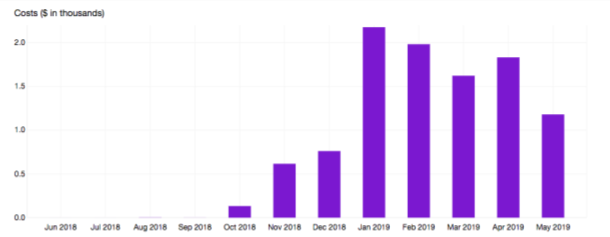
\includegraphics[width=\textwidth]{images/aws-metrics/total-cost.png}
\caption{AWS Total Costs\label{fg:awstotal}}
\end{figure}

\begin{figure}[!hbtp]
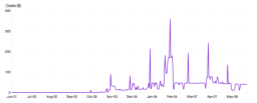
\includegraphics[width=\textwidth]{images/aws-metrics/total-cost-daily.png}
\caption{AWS Total Costs, daily\label{fg:awstotal}}
\end{figure}

\begin{figure}[!hbtp]
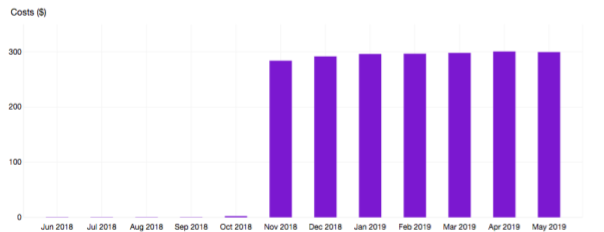
\includegraphics[width=\textwidth]{images/aws-metrics/s3-costs.png}
\caption{AWS S3 Costs\label{fg:awstotal}}
\end{figure}

\begin{figure}[!hbtp]
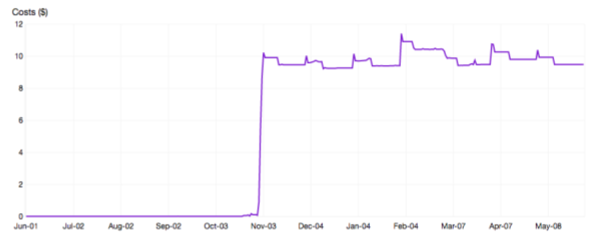
\includegraphics[width=\textwidth]{images/aws-metrics/s3-cost-daily.png}
\caption{AWS S3 Costs, daily\label{fg:awstotal}}
\end{figure}


\section{Local UVA HPC usage}
The Open Data Lab assists researchers in getting access to the local UVA HPC resources. For many of the tasks our users have there is no direct charge from local HPC and we do not track this usage. For more sustained efforts we do track the usage broken down by allocation.

The undergraduate UVA Machine Learning Club used up their entire initial allocation of 5,000\,SUs. They have been issued a new allocation of 100,000\,SUs. The results from one of their projects can be seen in section~\ref{sec:mlc}

The graduate UVA Machine Learning Club has used over half of their intial allocation. They have 3,335\,SUs used and 1,665\,SUs remaining.

\section{Sustained Support}
Many researchers are interested in using the Open Data Lab for continued hosting of their data sets to satisfy data management plan requirements of funding agencies. For example a federal agency that requires a seven year data commitment. In order for the open data lab to support this effort a budget model, at least in part, must provide for multi year sustained support.

\section{Funding Sources}
The ODL is funded by the DSI. The support for the Healthy Markets project is fronted by the ODL and then  cost transferred from the ODL PTAO to the HM PTAO.











